\section{Projectresultaat}
Het doel van de stageopdracht is om een draadloze sensor-probe te ontwikkelen die gebruikt kan worden in een proof-of-concept. Deze probes moeten in staat zijn om met reeds geselecteerde sensormodules dissolved oxygen (DO) te meten. Deze informatie moet draadloos verzonden worden en moet op een manier weer teruggekoppeld kunnen worden aan de regelmodule van de bioreactor. Dit systeem moet ook geïntegreerd worden in een testopstelling die duidelijk moet maken of de gewenste betrouwbaarheid van sensoren met kabels ook behaald kan worden door de draadloze probe.

\subsection{Systeemarchitectuur}
Als leidraad voor het vaststellen van systeemvereisten dient er een overzicht gemaakt te worden die duidelijk maakt uit welke (deel)systemen dit project bestaat en wat de scope van de ontwikkeling is tijdens dit project. Ook dient er duidelijk gemaakt te worden met welke bestaande systemen dit project te maken heeft, en in welke capaciteit.

\subsubsection{Systems Engineering}
Aan de hand van Systems Engineering is er een overzicht gemaakt van het gewenste systeem. In figuur \ref{fig:sensor_bdd} is een Block Definition Diagram (BDD) van het gewenste systeem te zien.

\begin{figure}[H]
	\centering
	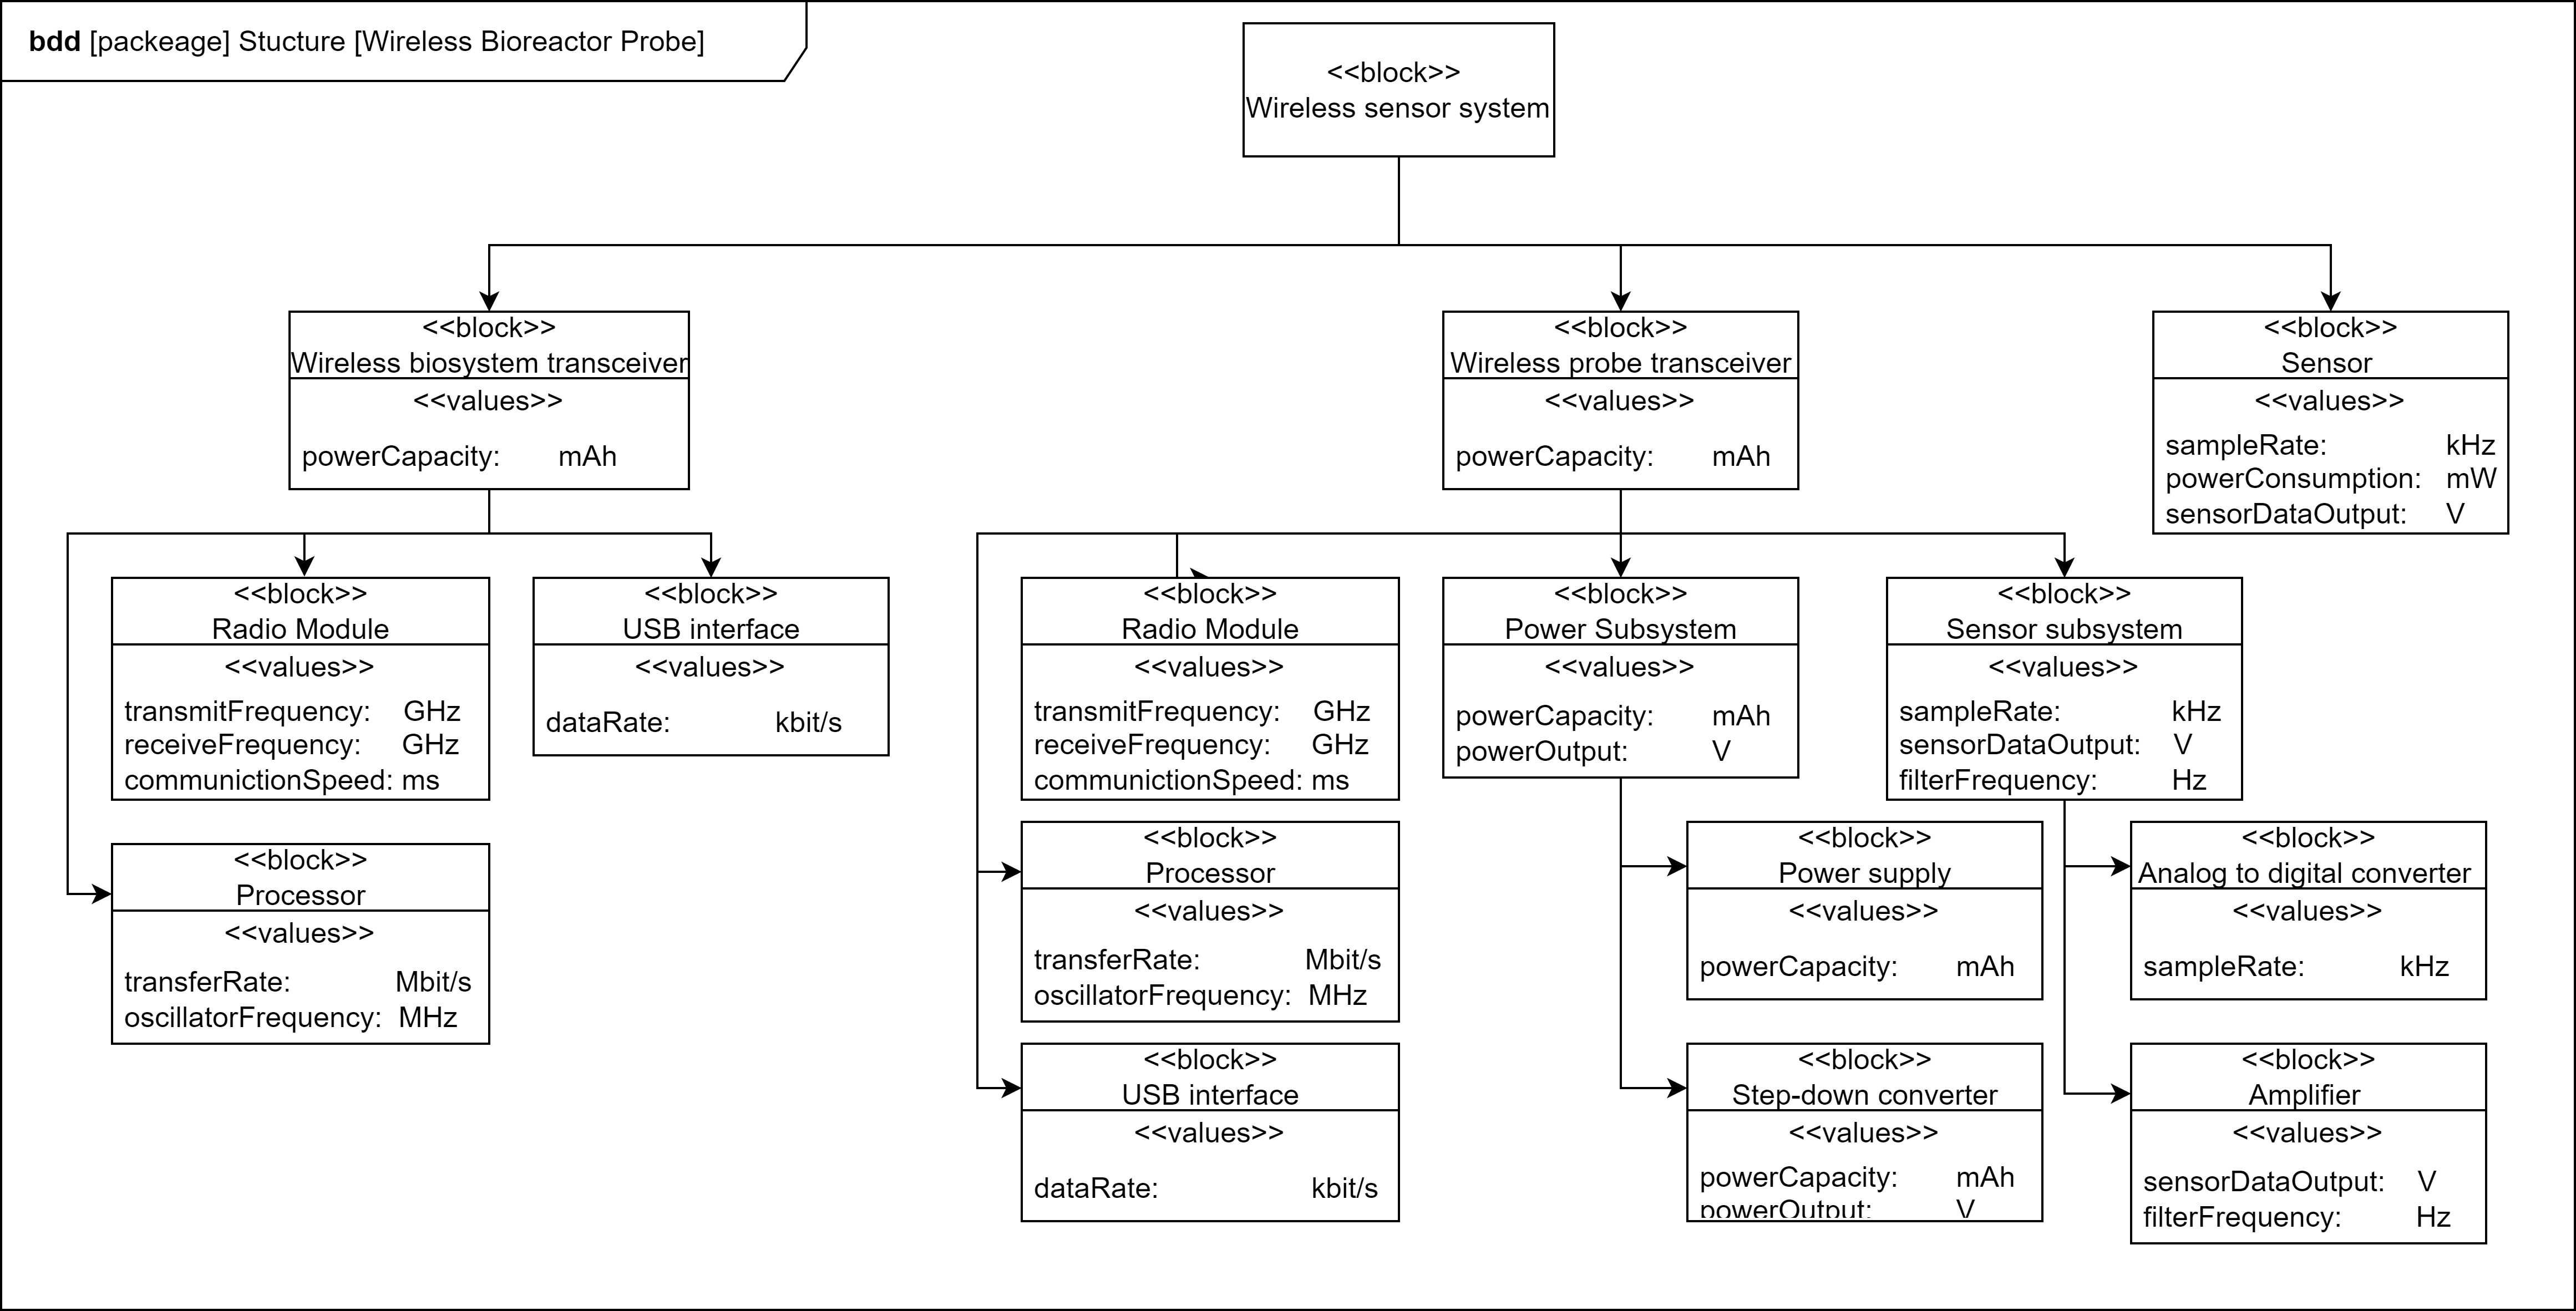
\includegraphics[width=1.0\linewidth]{graphics/sensor_bdd}
	\caption{Block definition diagram voor het draadloze bioreactor sensoren}
	\label{fig:sensor_bdd}
\end{figure}
In het BDD is te zien dat het wireless sensor systeem bestaat uit drie subsystemen: de biocontroller transceiver, de probe transceiver en de DO sensor. De biocontroller transceiver zal worden aangesloten op de biocontroller zodat het systeem kan communiceren met de DO sensor via de probe transceiver module. 

De biocontroller transceiver is een simpel systeem dat bestaat uit een draadloze module om met de andere probe te communiceren, een microcontroller om de data te verwerken en een USB interface om te communiceren met de biocontroller. 

De module voor de probe bestaat uit drie subsystemen: een draadloze module, een sensor module een een power systeem. Via de draadloze module kan de sensor data worden verzonden, de sensor module versterkt en digitaliseert het DO sensor signaal. Het power subsysteem verzorgt de probe en de module van stroom. 

Het doel van de probe transceiver module is om de bestaande analog to digital systeem te verfijnen en uit te breiden met een draadloze module. Het wireless bioreactor sensor systeem zal worden uitgerust met onder andere een processor om nodige sensor data te verwerken en de draadloze module aan te sturen.  

\begin{figure}[H]
	\centering
	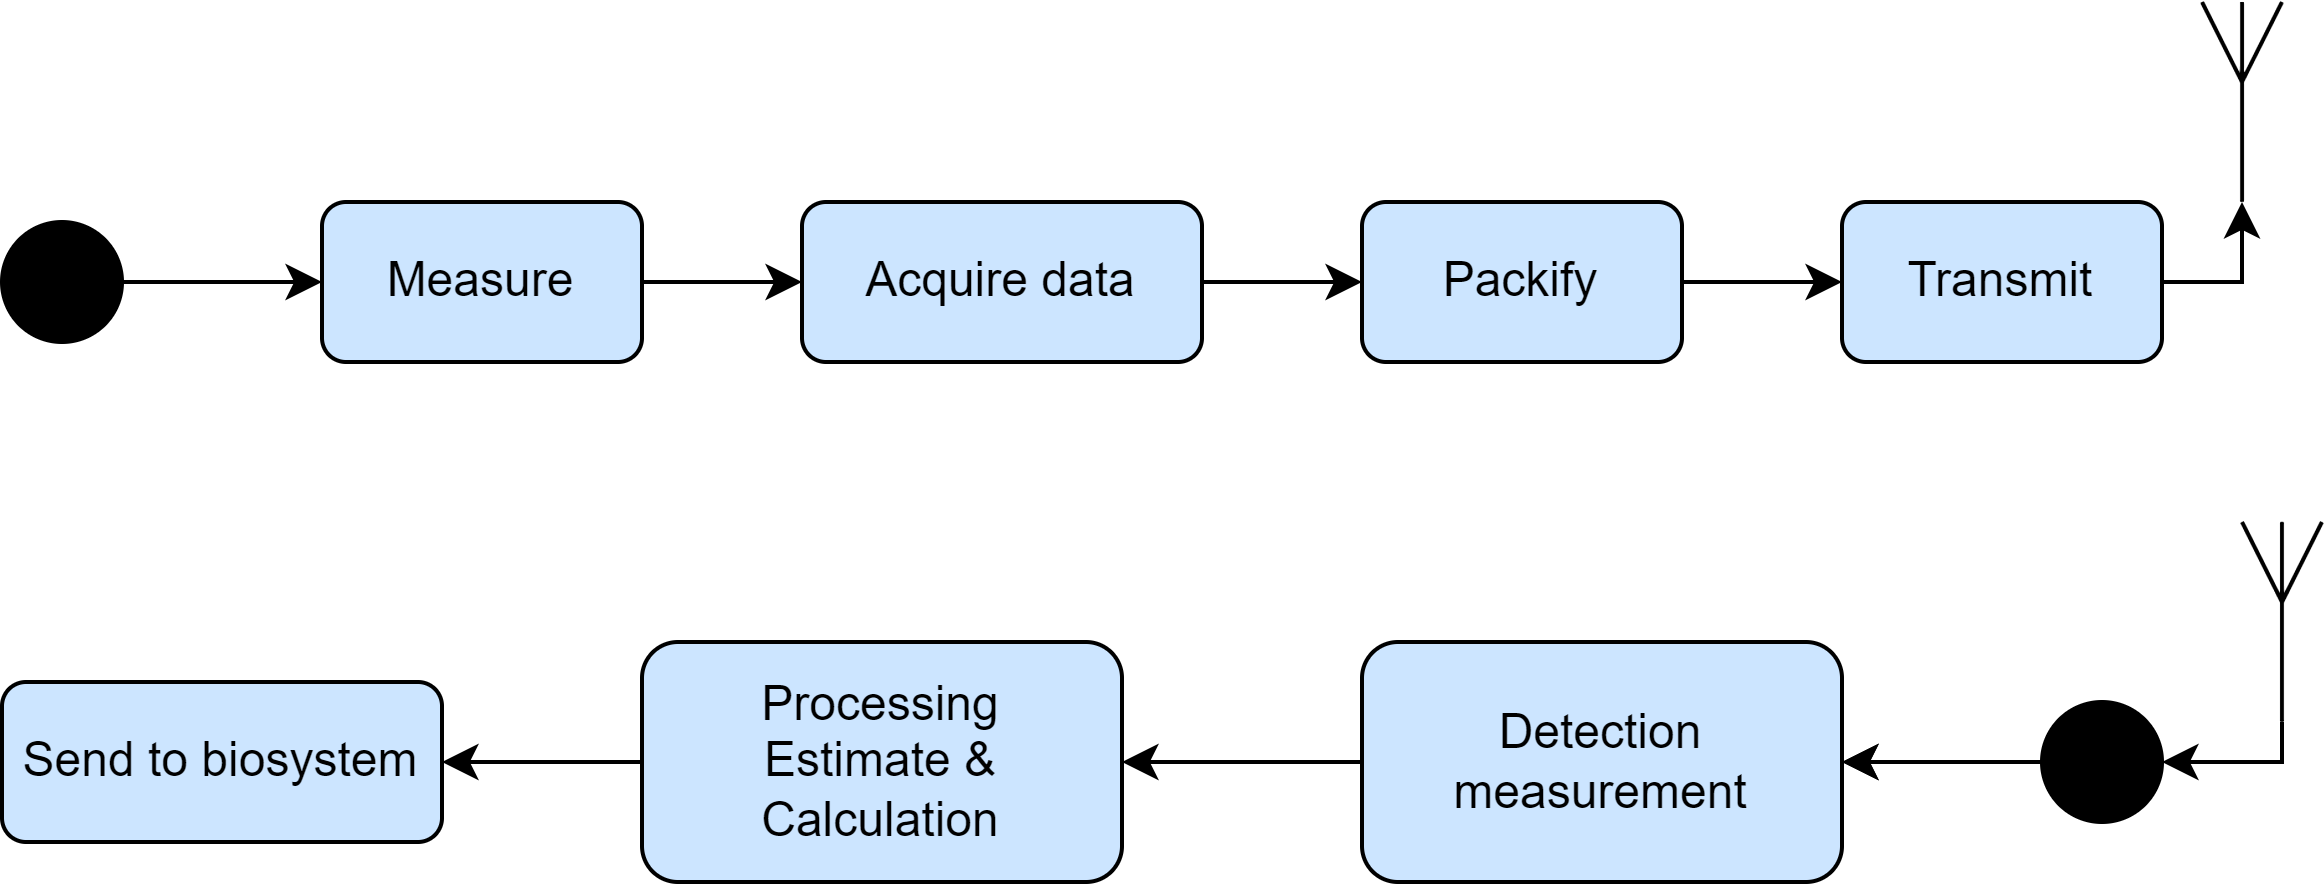
\includegraphics[width=0.60\linewidth]{graphics/probe_flow_simple}
	\caption{Flow diagram voor het draadloze bioreactor sensoren}
	\label{fig:probe_flow_simple}
\end{figure}

Figuur \ref{fig:probe_flow_simple} toont een flowchart van het verloop veen een DO meting. De meetcyclus start door het uitlezen van de de DO sensor. De data dat wordt verstuurd tussen de bioreator en biocontroller hebben een vast format, deze data pakketten worden verzonden door een transmitter. 

Na ontvangst door de receiver wordt de gemeten DO level omgezet naar een data format dat de biocontroller kan begrepen. 

Data acquisition wordt gedaan in een aantal stappen die zijn weergegeven in figuur \ref{fig:acq_flow}. Eerst zal het signaal worden gefilterd op een bepaalde frequentie. Via een opamp wordt het signaal geïnverteerd en doorgestuurd naar een analog to digital converter. Dit kan vervolgend worden uitgelezen en verwerkt via de microcontroller.  
\begin{figure}[H]
	\centering
	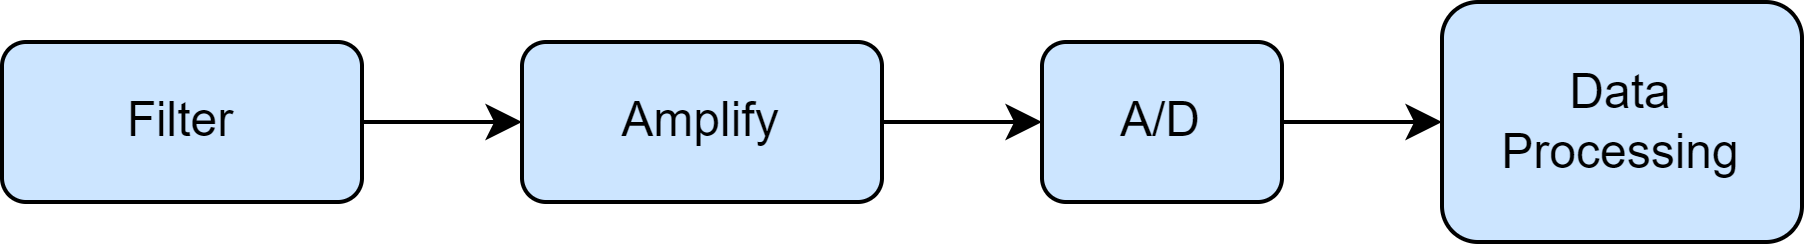
\includegraphics[width=0.55\linewidth]{graphics/acquisition_flow}
	\caption{Flow diagram voor het data acquisition van de bioreactor DO sensor}
	\label{fig:acq_flow}
\end{figure}


\subsubsection{Programma van Eisen}
Samen met de opdrachtgever, vertegenwoordigd door het engineeringsteam van Applikon, zijn er eisen aan het systeem gesteld. Op het moment van schrijven zijn de eisen nog niet gespecificeerd. Voor het pakket van eisen zal een apart document worden gemaakt waar de aanpassingen door de tijd heen ook worden vastgelegd. In tabel \ref{tab:PakketvanEisen} zijn de onderwerpen waar hoogstwaarschijnlijk een eis voor komt opgeschreven. 

\begin{table}[H]
	\centering
	\caption{Pakket van eisen.}
	\label{tab:PakketvanEisen}
	\begin{tabular}{clc}
		\toprule
		nr. & omschrijving  &  \\ 
		\midrule
		1 & sample rate &  \\
		2 & afmetingen behuizing &  \\
		3 & protocol output  &  \\
		4 & batterijduur &  \\
		5 & status indicatie &  \\
		6 & materiaal behuizing DO sensor a/d circuit &  \\
		\bottomrule
	\end{tabular}
\end{table}

Er zal een testplan worden opgesteld om te kunnen bepalen of er aan de eisen is voldaan. 